\chapter{Results}

\section{Performance}

\subsection{Measurements}

See Table \ref{table:resultFPS}, See Figure \ref{fig:performanceNodes}, See Figure \ref{fig:performanceLinks}

\begin{table}
    \centering
    \begin{tabular}{ | c | c | c | c | c | c | }
        \hline
        \textbf{nodes} & \textbf{links} &\textbf{layers} &\textbf{layout - FPS} &\textbf{expl. - min FPS} &\textbf{expl. - avg FPS}\\
        \hline
        310  & 0    & 3 & 40 & 90 & 90\\ \hline
        730  & 0    & 3 & 30 & 70 & 75\\ \hline
        1100 & 0    & 3 & 20 & 55 & 60\\ \hline
        1560 & 0    & 4 & 20 & 40 & 55\\ \hline
        2343 & 0    & 5 & 10 & 30 & 35\\ \hline
        774  & 387  & 3 & 20 & 60 & 70\\ \hline
        774  & 1548 & 3 & 20 & 55 & 70\\ \hline
        774  & 3870 & 3 & 10 & 40 & 60\\ \hline
        1560 & 3120 & 4 & 5  & 25 & 45\\ \hline
        1020 & 2040 & 4 & 10 & 40 & 60\\ \hline
     \end{tabular}
     \caption{Results from performance measurement evaluation(expl. ... exploration).}
     \label{table:resultFPS}
\end{table}


\begin{figure}[h]
    \centering
    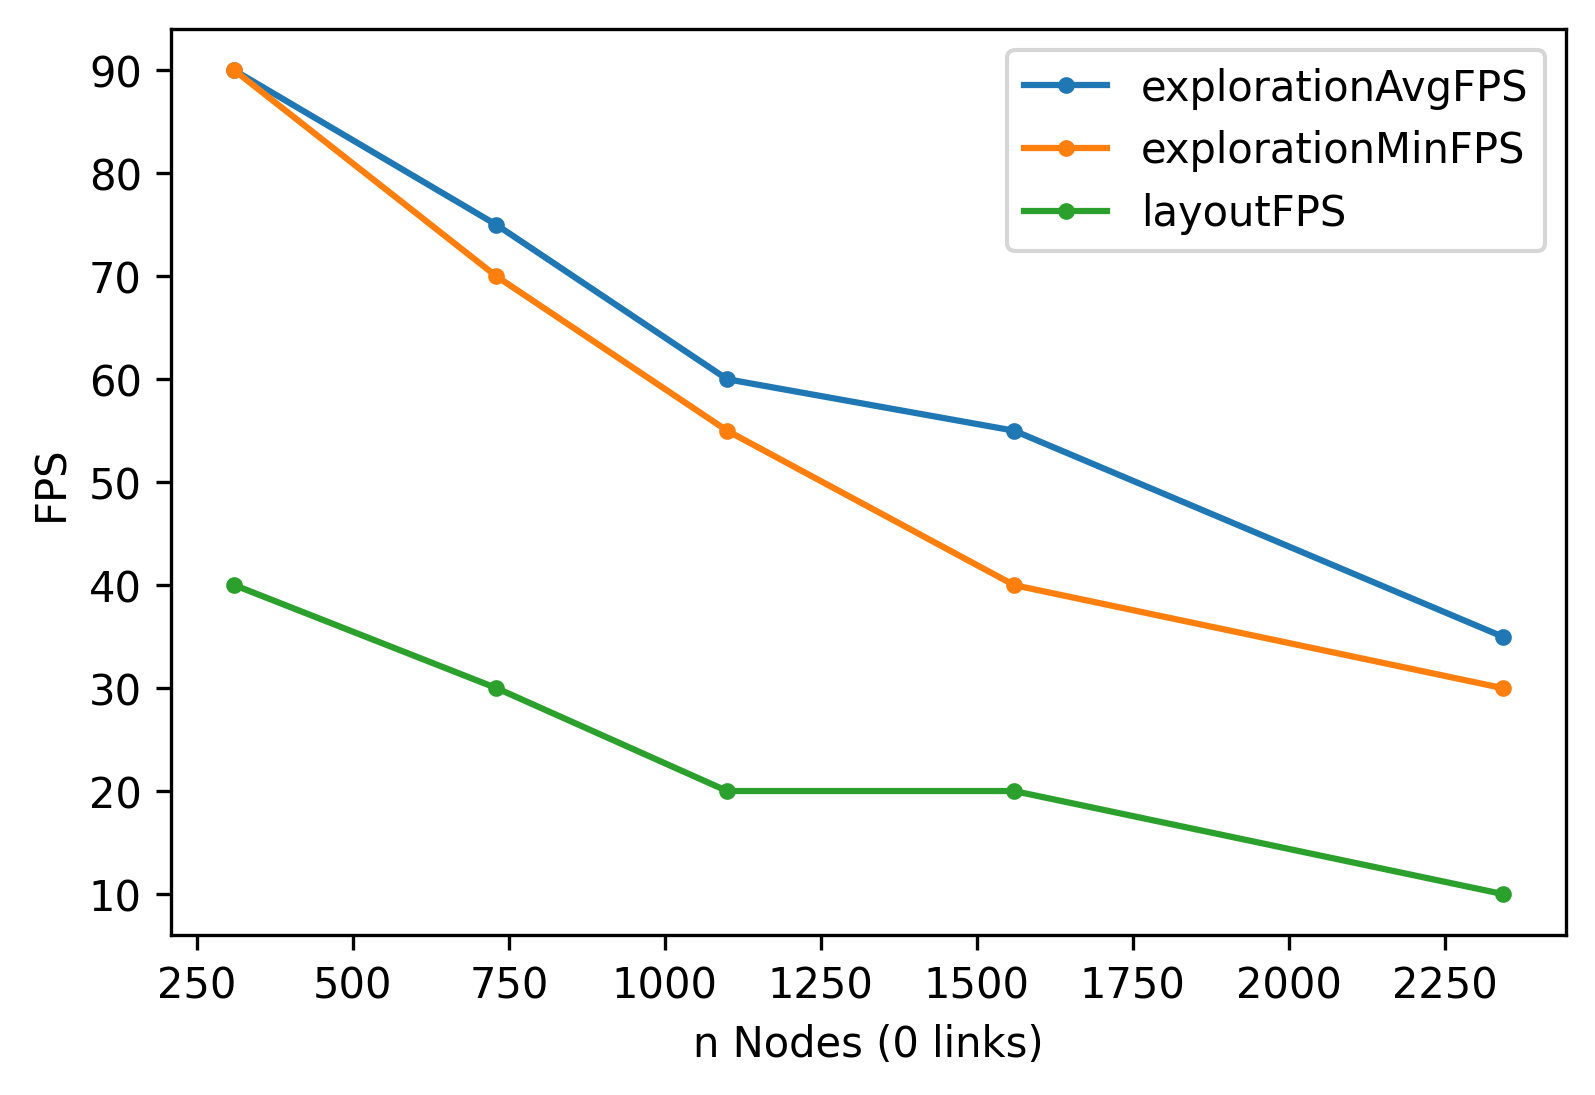
\includegraphics[width=0.75\textwidth]{graphics/performanceAnalysisNodes.png}
    \caption{Performance chart for scaling the number of nodes.} 
    \label{fig:performanceNodes} 
\end{figure}

\begin{figure}[h]
    \centering
    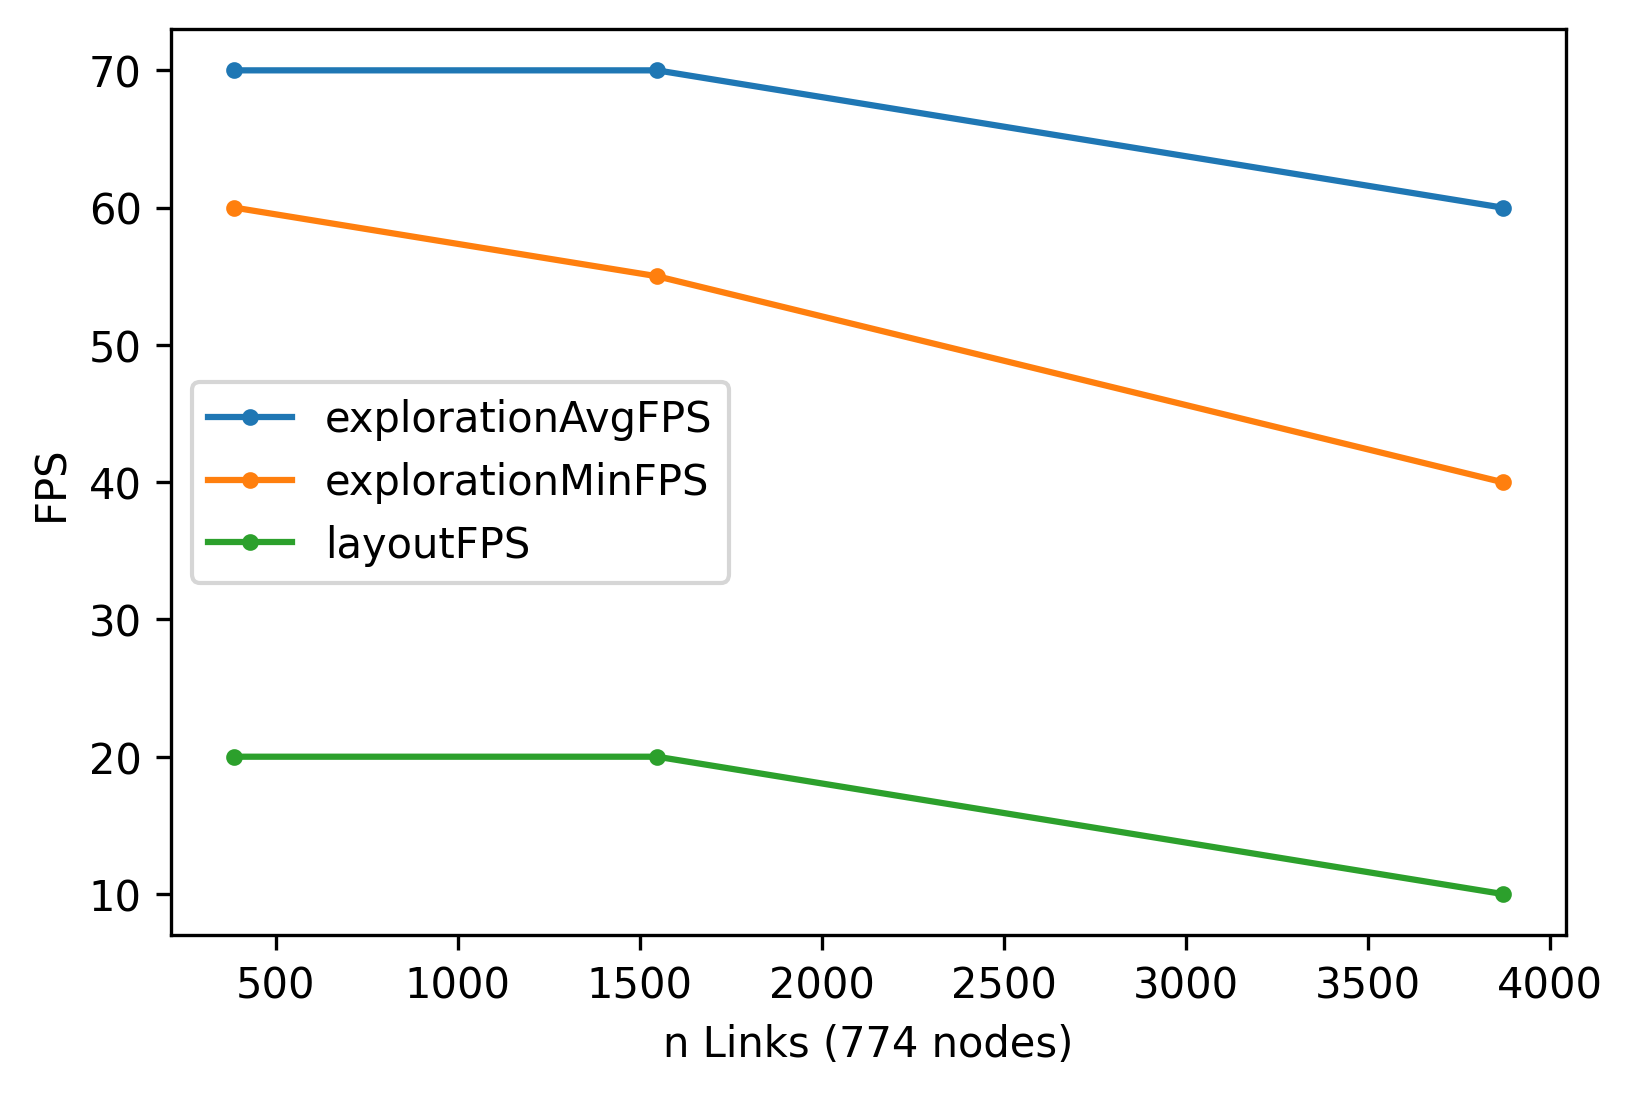
\includegraphics[width=0.75\textwidth]{graphics/performanceAnalysisLinks.png}
    \caption{Performance chart for scaling the number of links.} 
    \label{fig:performanceLinks} 
\end{figure}

\subsection{Possible optimization}


\section{Informal feedback}

\subsection{Clarity of the visualization}
Filtering, visual clutter, hierarchical layout(intuitive?), ...

\subsection{Navigation}
Free fly, animated teleport, scaling, motion sickness.

\subsection{Interaction}
Button Mappings, Laser Pointer, 

\subsection{Performance}
Tested system and dataset